% vim:set et sw=2 ts=4 tw=72:
\chapter{Background and Related Work}\label{chap:background}

A version control system tracks files, and how they are changed over
time.
While it can be used for storing any digital information,
version control is usually used in the context of software development;
it is used for storing and managing the files of the project, including
the project's source code and binary assets.
Version control has two primary purposes: first as a means of storing
files, and second as a means of retrieving historical versions of those
files.
In addition to fulfilling the two primary purposes, a version control
system maintains a log of who is making the changes and when the
changes were made.

Early version control systems, such as Revision Control System (RCS),
were designed for local development and provided no means of collaboration.
As software projects grew, the model quickly became outdated,
being replaced with a centralized server model.
Concurrent Version System (CVS) and Apache Subversion (SVN) are two
examples of centralized version control systems. The centralized version
control system provides means of collaboration through a client-server
interface. The repository is stored in a central server. Developers use
a client to check out parts of the repository, choosing parts that
pertain to the part they are editing.

In large open source projects, the centralized architecture becomes a
burden. Common tasks such as committing and changing branches requires
re-synchronization with the central server.
To work with the repository,
the developer must always have access to the central server.
To maintain the atomic properties of committing, the server will
momentarily lock the repository to ensure that no other changes happen
while a commit is being processed or a conflict resolved.

Due to the limitations of a centralized architecture, the Linux kernel
uses a distributed version control system. Until April of 2005, the
kernel project used BitKeeper.
In April 2005, the licensing became too restrictive and Linux was forced
to change version control systems. \evantodo{Find a reference}
Git was written as the replacement for BitKeeper, and was designed to
maintain a similar level of patch granularity as in BitKeeper\footnote{
  initial announcement of git on the mailing list
  \url{https://marc.info/?l=linux-kernel&m=111280216717070}}. The first
version of git was roughly 1300 lines of code and was written and
self-hosting in less than two weeks\footnote{From the git mailing list
  \url{https://marc.info/?l=git&m=117254154130732}}.

Both BitKeeper and git are distributed version control systems (DVCS).
In distributed version control, the entire repository is mirrored on
the developer's local computer instead of copying parts of the project.
As a result, the local copy is much larger on disk than with a
centralized repository, but the developer has the freedom to make
changes to the code and to the
structure of the repository without needing to re-synchronize with a
central server.

It is often desirable to have the features of version control available
before a feature is ready to be made available in a public-facing
repository.
It is also desirable that the commits into the master branch of the
master repository leave the project in a state that will both compile
and operate correctly.
Distributed version control makes this possible; developers can combine,
split, and edit commits locally before pushing their changes into the
central repository.

Cloning is when a developer copies a repository.
The source repository is recorded as a remote repository.
It is possible for repositories to have many remotes.
The process of updating a remote repository with the changes made in the
local repository is known as pushing.
By default, the remote repository that was cloned will be given the
label \textit{origin}, which is the repository where git will push to
and pull from, unless another remote is specified.

After changes are made to a remote, the local repository must
resynchronize with the remote in order for those changes to be
propagated.
This resynchronization can be done in one of two ways.
The normal way of resynchronizing is through the \textit{pull} command,
which fetches the changes in the origin repository, then merges the
branches of the origin repository into the corresponding branches in the
local repository.
The second way of resynchronization breaks the process into two steps,
manually issuing the fetch command and then manually merging or rebasing
branches.
Rebasing is the process of moving one or more commits from one ancestor
to another.

The process of updating a remote repository with the changes made in
the local repository is known as pushing.
If there are no merge conflicts, the merge can perform a fast-forward
merge, shown in Figure~\ref{fig:fast_forwarded_merge},
which flattens the changes made in the origin repository into the
master branch of the local repository.
Fast-forward merging hides the fact that git would otherwise consider
the two repositories to be separate branches.
Without fast-forward merging, any resynchronization would result in the
addition of a new merge node.
If there is a merge conflict, or the user has specified that the merge
should not fast-forward, a merge commit is created, as shown in
Figure~\ref{fig:merge_node_merge}.

\begin{figure}[htpb]
  \centering

  \begin{subfigure}[b]{0.5\textwidth}
    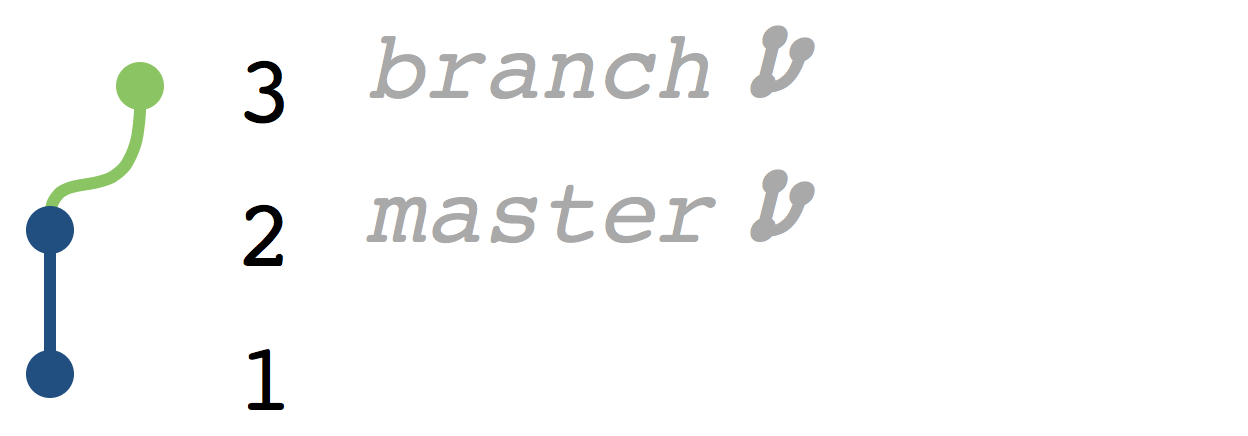
\includegraphics[width=0.85\textwidth]{Figures/background/fastforward/fastforward_2.png}
    \caption{The repository contains two commits that are part of the
      master branch, with one commit that is part of a separate branch
      waiting to be merged.}
  \end{subfigure}

  \begin{subfigure}[b]{0.5\textwidth}
    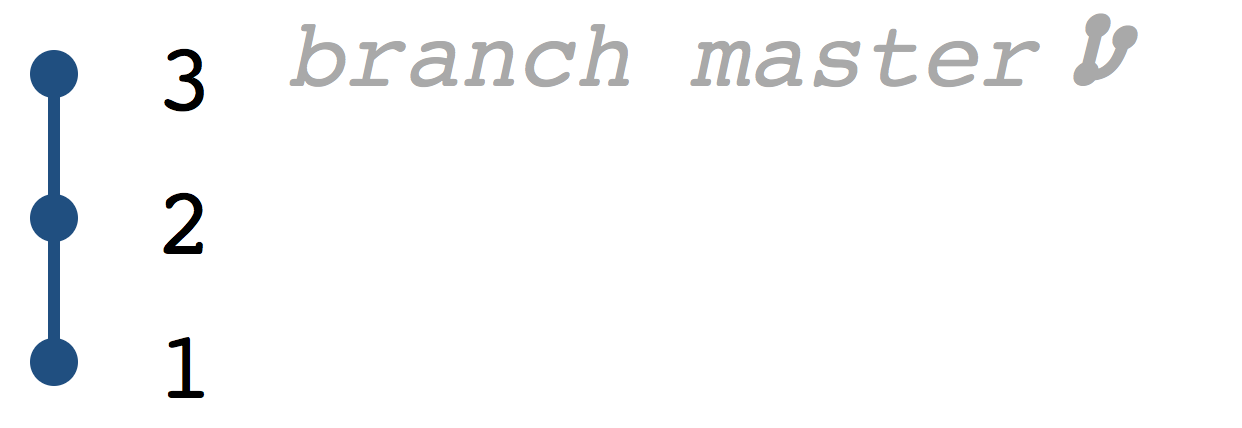
\includegraphics[width=0.85\textwidth]{Figures/background/fastforward/fastforward_3.png}
    \caption{A fast-forward merge does not create a merge commit,
      and instead moves the branch pointer forward to the branch pointer.}
    \label{fig:fast_forwarded_merge}
  \end{subfigure}

  \begin{subfigure}[b]{0.5\textwidth}
    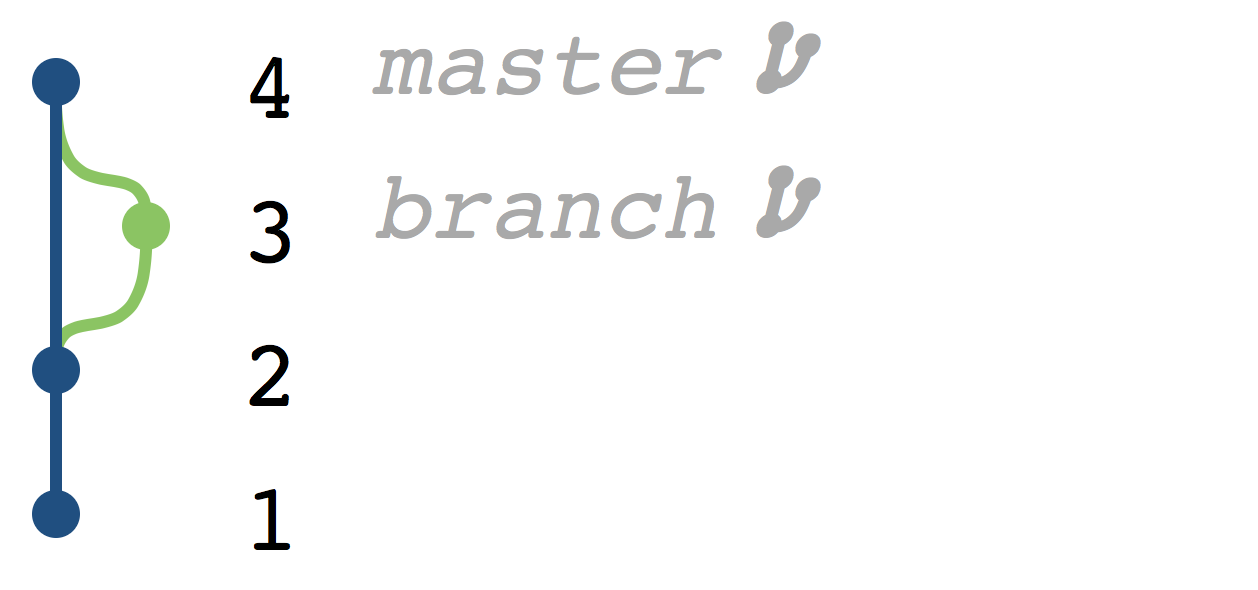
\includegraphics[width=0.85\textwidth]{Figures/background/fastforward/fastforward_4.png}
    \caption{A merge commit is created when the merge cannot be made
      cleanly, or \textit{--no-ff} is passed to the merge command.}
    \label{fig:merge_node_merge}
  \end{subfigure}
  \caption{A depiction of the distinction between fast-forward merges
    and non fast-forward merges}
  \label{fig:merge_styles}
\end{figure}

Distributed version control gives developers more flexibility with their
local repository and requires the developer to synchronize their local
copy of the repository with the public master repository less often
than with centralized version control.
The public master repository can be thought of as being the equivalent
of the central repository in a centralized system.
Instead of it being enforced by the version control system,
it is a socially agreed upon location where the official version of the
code exists.
Unlike with the centralized version control though,
there is no requirement for the developer to ever push their changes
back to the public repository;
the local repository is completely standalone.
Developers can make changes that would otherwise break the workflow of
other developers because they have a standalone repository.
These changes include rebasing branches, re-ordering commits,
splitting commits, and squashing commits into one.
Once the developer is happy with their set of commits, they may push
them to the remote repositories.

Git needs to be designed to handle multiple repositories, with many
developers working simultaneously.
It also needs to be able to support the ability to move commits between
branches, re-order commits, combine multiple commits into a single
commit, and split a commit into multiple commits.

To support these requirements, Linus chose to use a directed acyclic
graph to represent the commits and the relationships between commits.
The graph imposes relatively few constraints on what a developer can do.
The only requirement is that there is not a cycle in the commits, that
is, a change that at some point depends on itself.
For example, SVN always has a well-defined trunk, the SVN equivalent of
a master branch, whereas git does not require the existence of a master
branch.
The graph structure also supports relatively cheap braching compared to
other version control systems, which makes it possible for developers to
create more branches without having to worry about consuming excessive
resources.
With fewer constraints on the structure of the commit graph in git,
tools are unable to make as many assumtions when abstracting the graph.
Many tools avoid this by not abstracting the graph and visualizing other
properties of the repository, such as the file structure.
Tools that do visualize the graph do only minimal abstraction, creating
a visualization of the graph itself.

The graph of large and active repositories is very complicated.
It is very difficult to understand the relationship between commits, and
how the commits are integrated into the project from a visualization of
the graph.
This poses a problem for a maintainer who must understand how a
commit is integrated into the master branch of a
project and the other commits that are integrated with that commit.
Maintainers must sift through thousands of commits to determine which
changes being made to the current version of the software pertain to
the area of the software that they are maintaining.
Specifically, maintainers must be able to answer two questions:

\begin{textbox}
\begin{itemize}
  \item How is a commit integrated into another branch?
  \item What other commits are integrated with the commit?
\end{itemize}
\end{textbox}

The remainder of this chapter includes related work, a description of
git, the directed acyclic graph used internally by git, and information
about the Linux kernel repository.

\section{Related Work}\label{sec:related_work}

A Version Control System (VCS) tracks the development of a software project,
recording each change as it happens. By tracking the changes, the VCS
contains the entire history of the software, rich with information about
who the authors are, what files are being modified, and the changes
being made.
This makes the VCS vital in providing information about
how a software project is being developed and how the software is
structured. In order to use the information stored in the VCS, users
must be able to gain a clear understanding and summarization of the
changes being made, and how they interact with the rest of the source
code. While there has been extensive research on visualizing software
repositories, previous work does not focus on how commits and merges are
structured in the repository graph, and in extension, how commits are
integrated into a repository.

The literature on repository visualization
and summarization can be broken down into three academic subcategories:
communication\cite{Cubranic2005,Begel2010}, aspect-oriented
visualization\cite{Ambros2005,Burch2005,Ambros2009}, and organic
visualizations\cite{ogawa09,Caudwell2010}.\evan{I don't know what you
  mean by "be consistent" here, I don't see the inconsistency.}
A fourth industrial category exists, including tools like GitKraken and
SourceTree.
The goal of the industrial tools is not to extract or synthesize new
information from the repository, but to act as a user-friendly client
on top of what git already provides.

Many tools focus on addressing the issue of communication between
developers in inter-team collaborative work. Hipikat\cite{Cubranic2005}
investigated communication between developers, focusing on assisting
with the integration of new developers into a project though
communication, providing the new developer with searchable artifacts of
the changes being made, and where to find them. The artifacts may
include files or bug information, shown in Figure~\ref{fig:hipikat}.
Codebook\cite{Begel2010} also focused on communication, but while
Hipikat focused on assisting new developers find artifacts, Codebook
assists developers with finding who was responsible for creating the
artifact. Codebook used a data-mining technique to determine the
developer of a piece of code, the program manager who wrote the
specification for the code, and the program managers and developers on
the team who were working together. A screenshot of Hoozizat, an
implementation of Codebook, is shown in Figure~\ref{fig:codebook}.
Hoozizat and Hipikat use the version control as the archive of artifacts
that are being queried. Neither tool is designed with the goal of
providing information on the topological structure of a source code
repository, nor are these tools designed for visualization purposes, but
they do draw information from the contents of the version control
system.

\begin{figure}[htpb]
  \centering
  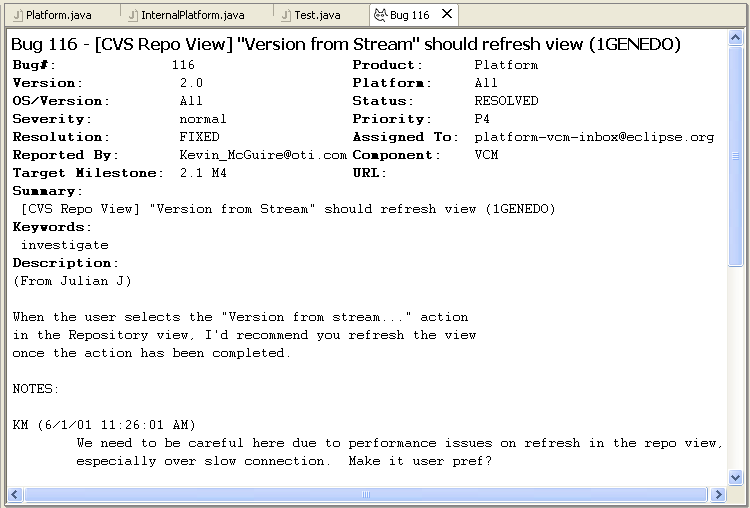
\includegraphics[width=0.9\linewidth]{Figures/introduction/hipikat_bug.png}
  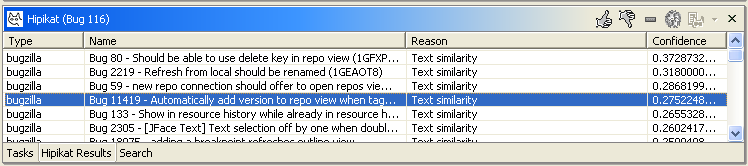
\includegraphics[width=0.9\linewidth]{Figures/introduction/hipikat.png}
  \caption{View of Hipikat, listing bugs that are similar to the one
  being viewed}
  \label{fig:hipikat}
\end{figure}

\begin{figure}[htpb]
  \centering
  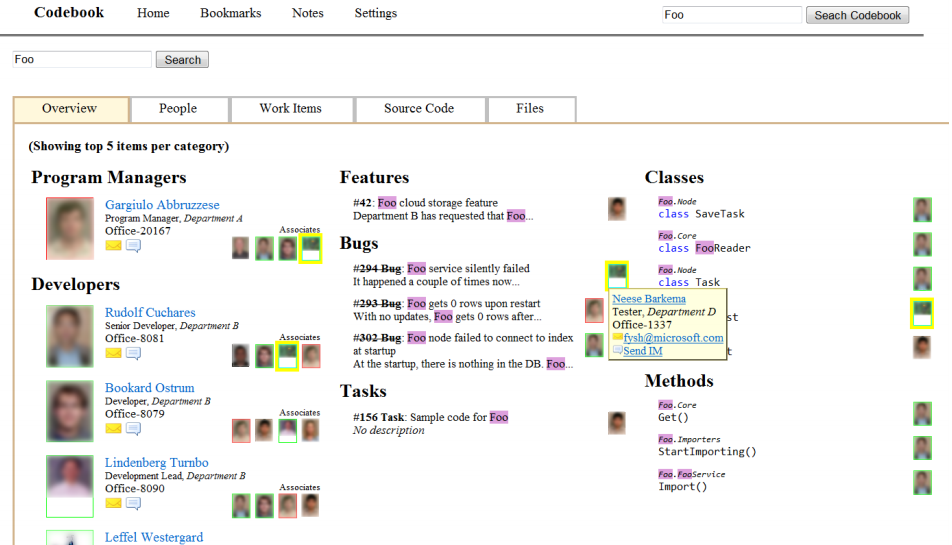
\includegraphics[width=0.8\linewidth]{Figures/introduction/codebook.png}
  \caption{A screenshot of the search results on Hoozizat, an
    implementation of codebook.}
  \label{fig:codebook}
\end{figure}

Most visualization systems provide information about a certain aspect of
the contents in the repository. The goal of Fractal
Figures\cite{Ambros2005} is to show the division of work between
contributors. The project is represented as a square. The square is then
subdivided based on the proportion that a given contributor contributed
to the project, shown in Figure~\ref{fig:fractal_figures}. The
visualization makes it easy to see where work is evenly divided versus
the projects where a single contributor is doing most of the work.

\begin{figure}[htpb]
  \centering
  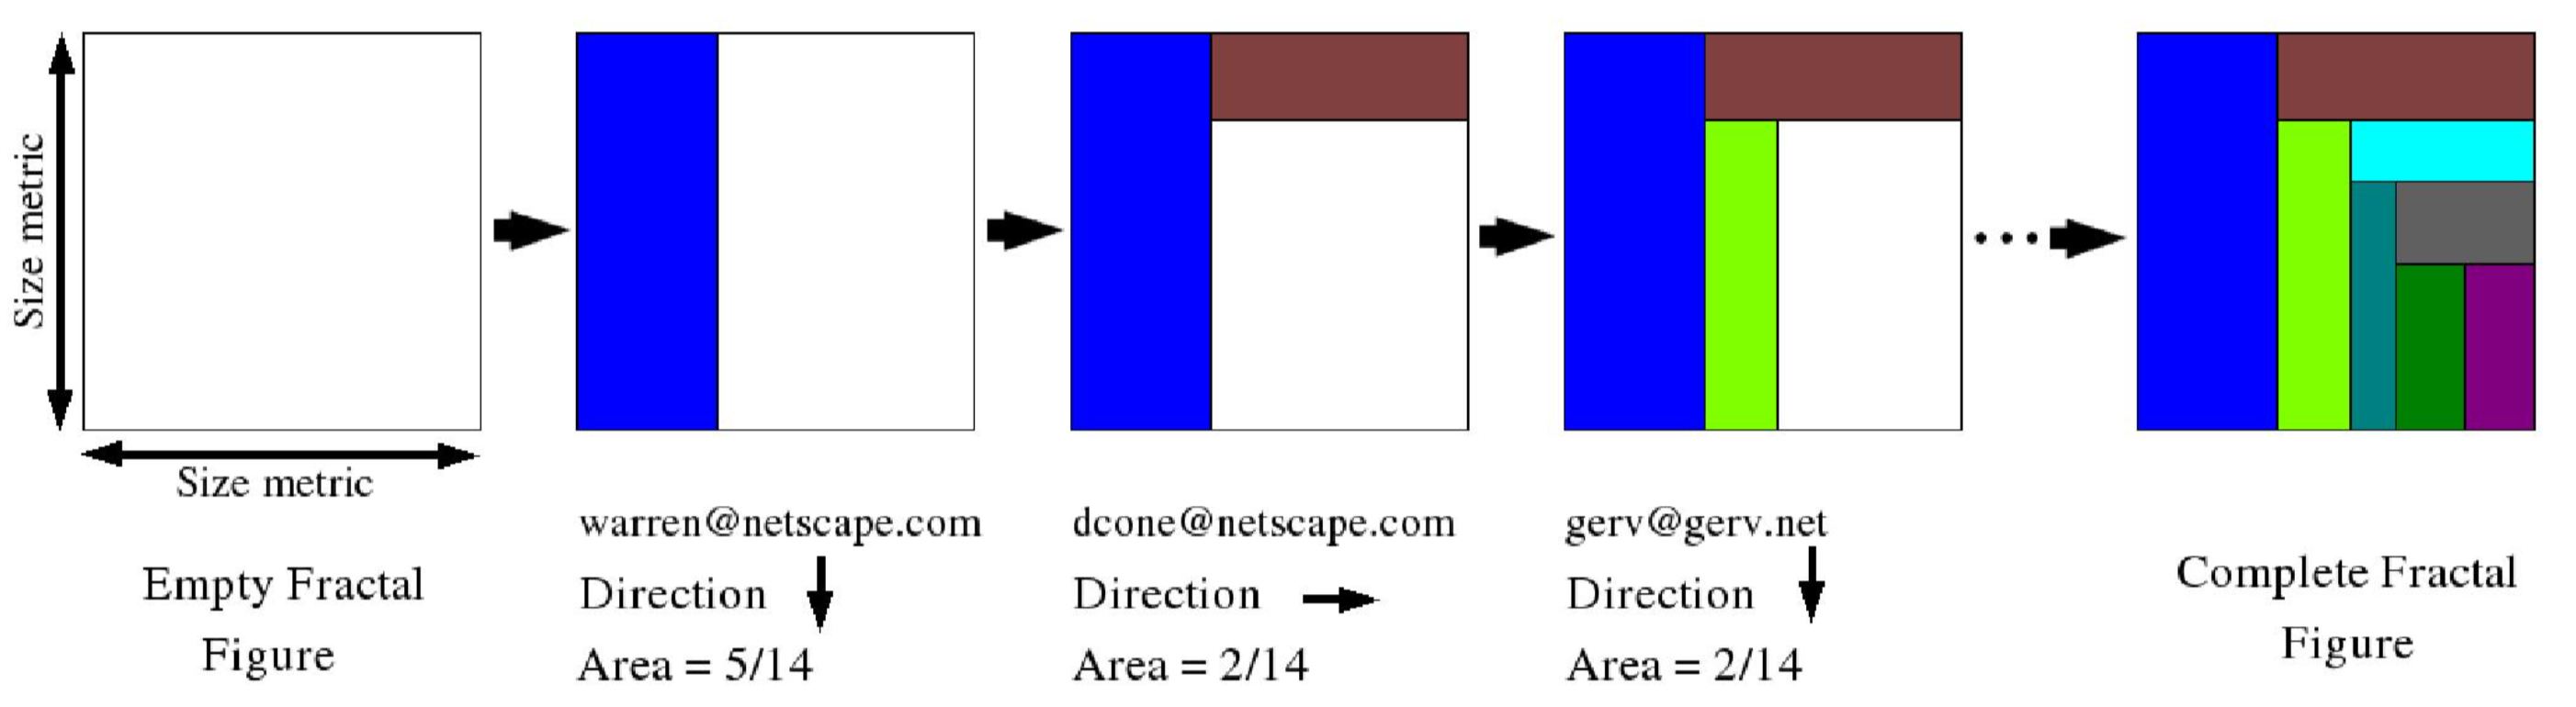
\includegraphics[width=0.8\linewidth]{Figures/introduction/fractal_figures.png}
  \caption{Construction of Fractal Figures}
  \label{fig:fractal_figures}
\end{figure}

EPOSee\cite{Burch2005} and Evolution Radar\cite{Ambros2009} use the
information from the version control system to determine which files
are edited together.
These tools  are designed to help a user identify the degree to which
two files are coupled.
Two files are edited and committed together frequently are said to be
more tightly coupled.
This makes it possible to determine when two classes are semantically
related.
The evolution radar shown in Figure~\ref{fig:evolution_radar} places
points on a circle based on the name and coupled they are.
The files are arranged around the circle
based on the file name, including the full file path. This has the
effect of grouping files that are from the same directory. The distance
from the center of the circle is dependent on how tightly coupled the
file is to the file be analyzed. A more tightly-coupled file will be
positioned more closely to the center of the circle.

\begin{figure}[htpb]
  \centering
  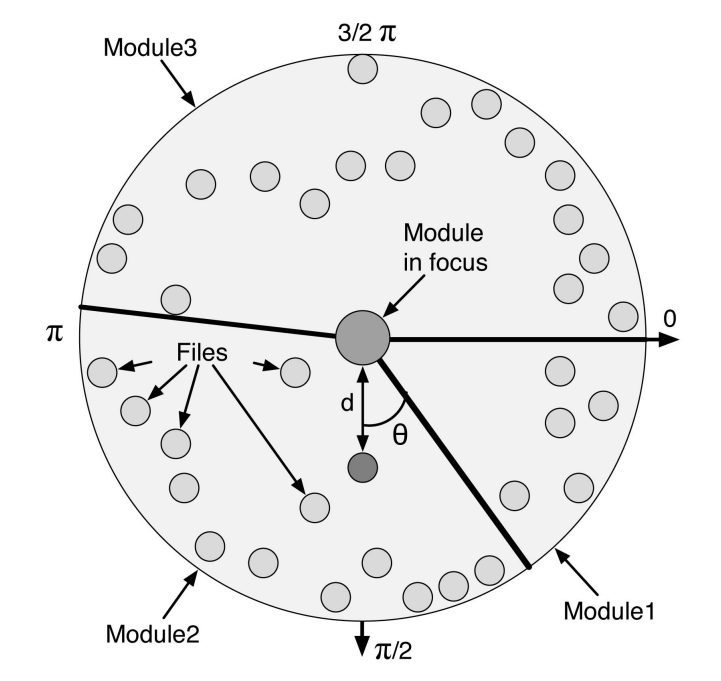
\includegraphics[width=0.8\linewidth]{Figures/introduction/evo_radar.png}
  \caption{Evolution Radar visualization}
  \label{fig:evolution_radar}
\end{figure}

Hoozizat, Hipikat, Fractal Figures, EPOSee, and Evolution Radar all
extract data from CVS repositories. Our goal is to provide information
about git repositories. Fewer tools are available for generating
visualizations and summaries of git repositories.

Organic visualizations show patterns in cooperation and communication
that arise within a software project organically\evan{One definition of
  Organically: When something happens naturally without planing and is not forced.}.
Heller et al.\cite{Heller2011} plots communication on a map.
This visualization show patterns in communication as the arise, and how
these communication channels operate internationally within a software
project, depicted in Figure~\ref{fig:heller_map}.

\begin{figure}[htpb]
  \centering
  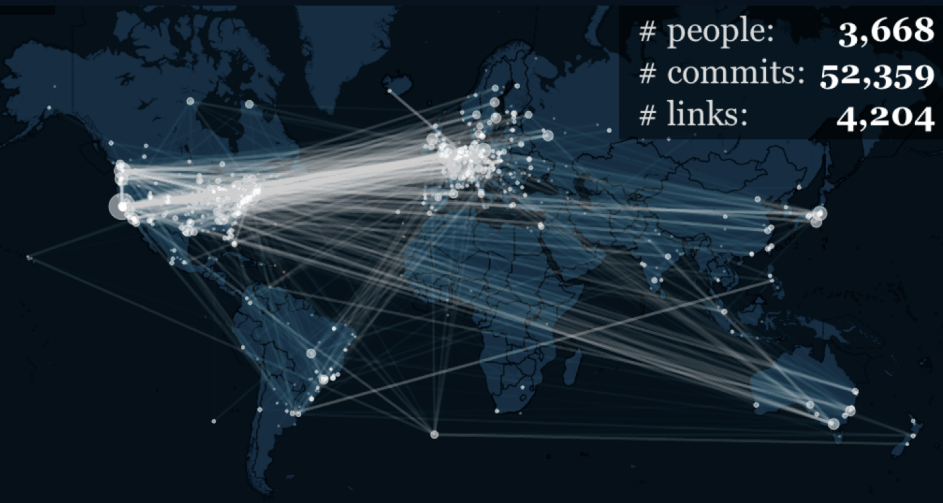
\includegraphics[width=0.8\linewidth]{Figures/background/heller_map.png}
  \caption{A screenshot of the communication mapping tool by Heller et
    al.\cite{Heller2011}}
  \label{fig:heller_map}
\end{figure}

The visualizations proposed in Gource\cite{Caudwell2010}, shown in
Figure~\ref{fig:gource_view}, shows which files contributors are working
on.
Using this, it is possible to draw conclusions about which parts of a
project a given contributor is working on and the group of contributors
working on a given area. Gource uses a graph metaphor structure to
represent the file structure of a repository. Files in the same
directory cluster together to form a node. Edges between the directory
clusters represent which directory contains another, although there is
no way to determine the direction of the relationship.
User avatars move around the graph emitting different beams of colored
light depending on the change being made to the file.
Green indicates the creation of a new
file, yellow indicates a modification, and red indicates the deletion of
a file. The visualization is animated to show how a project grows over
time. Codeswarm\cite{ogawa09}, shown in Figure~\ref{fig:codeswarm}, is
similar to Gource, using a timelapse approach to visualizing the events
in the repository.
Unlike Gource, which constructs a graph from the directory structure
of project, Codeswarm does not have a graph structure;
developers are the center of the visualizations.
When a developer makes a change to a file, the file lights up and
flies toward the developer.
As a developer makes more changes, the files that the developer is
modifying will form a ring around the developer.
If multiple developers are modifying a file, the developer nodes
are drawn together.

\begin{figure}[htpb]
  \centering
  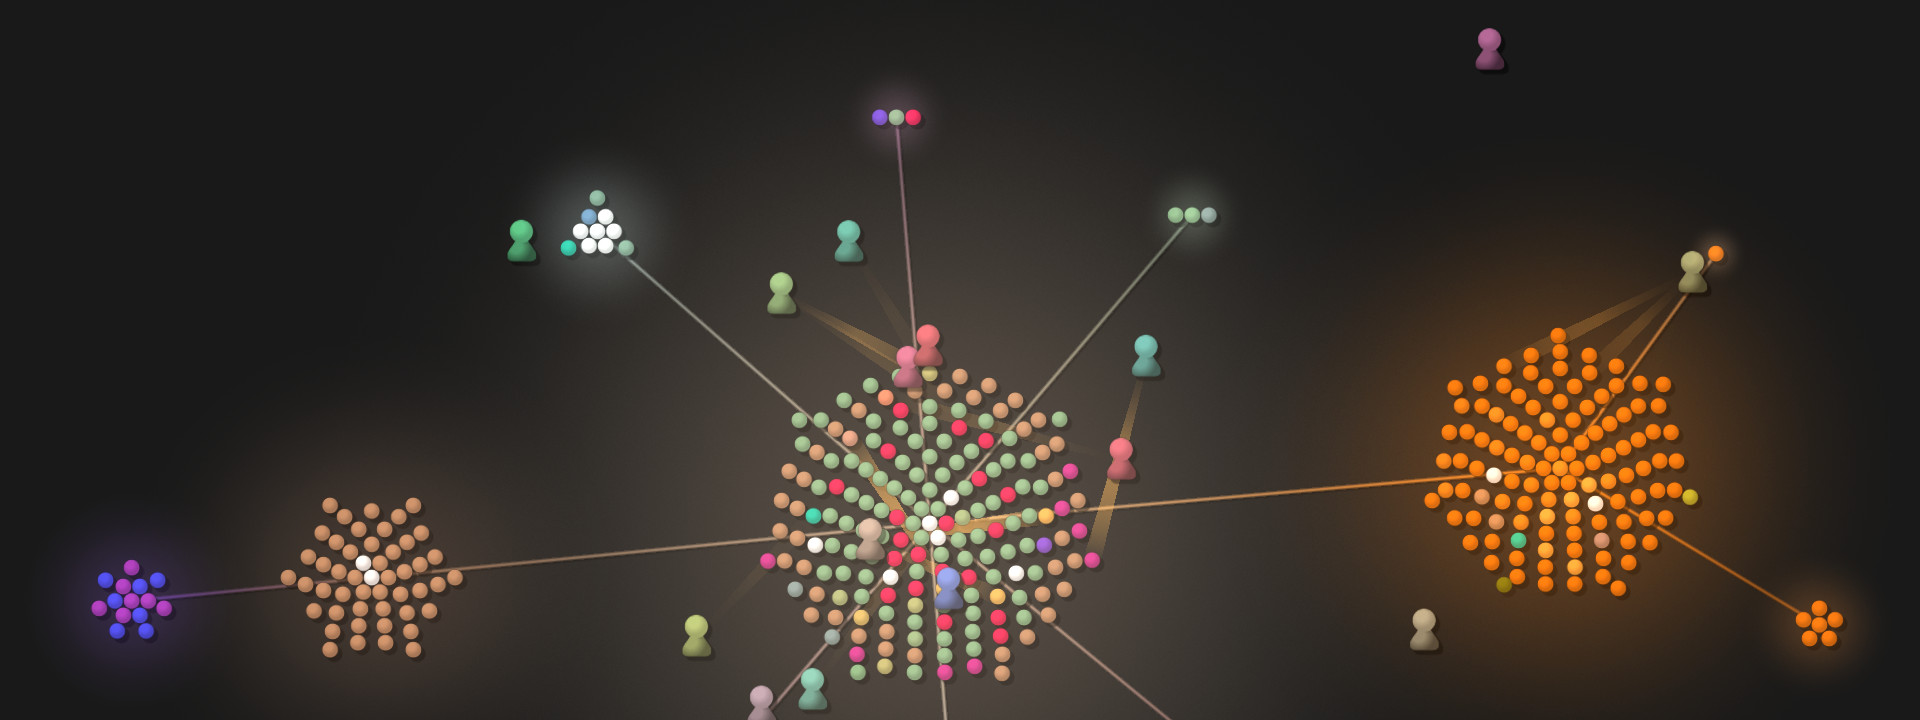
\includegraphics[width=0.8\linewidth]{./Figures/introduction/gource-linux.jpg}
  \caption{View of Gource file graph with users operating on a
    repository}
  \label{fig:gource_view}
\end{figure}

\begin{figure}[htpb]
  \centering
  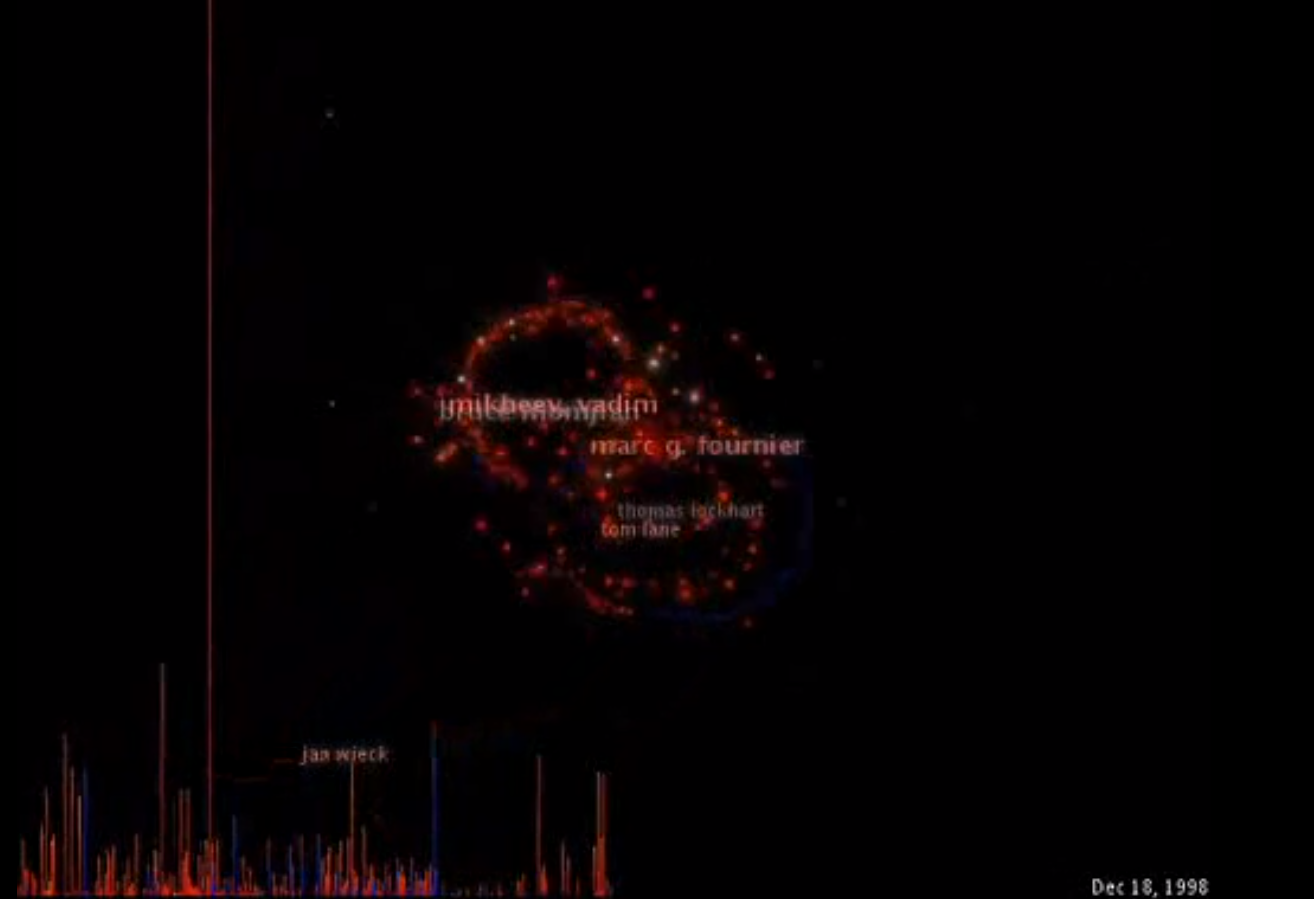
\includegraphics[width=0.8\linewidth]{Figures/introduction/codeswarm.png}
  \caption{View of the Postgresql repository in Codeswarm}
  \label{fig:codeswarm}
\end{figure}

There are many non-academic tools that are designed as an interface to
git.
While not all of these programs provide visualizations, those that
do use a visual metaphor of the DAG to show topological relationship
between commits.
While they ultimately show the same information, the topology of the
repository, the organization of that information is different.

GitKraken, shown in Figure~\ref{fig:gitkraken_main},  is a popular
commercially written git interface that aims to be efficient, elegant,
and reliable, according to it's official website.
On visual inspection, it appears to satisfy these goals.
Overall, the interface is clean and most actions that are possible with
the git command line are available in the graphical interface.
The tool is effective and garners online approval from users.
The graph of the commits is shown in the center of the main view and
provides users with the same information as the graph visualization in
gitk and the git command line, though it may be visually more appealing.

\begin{figure}[htpb]
  \centering
  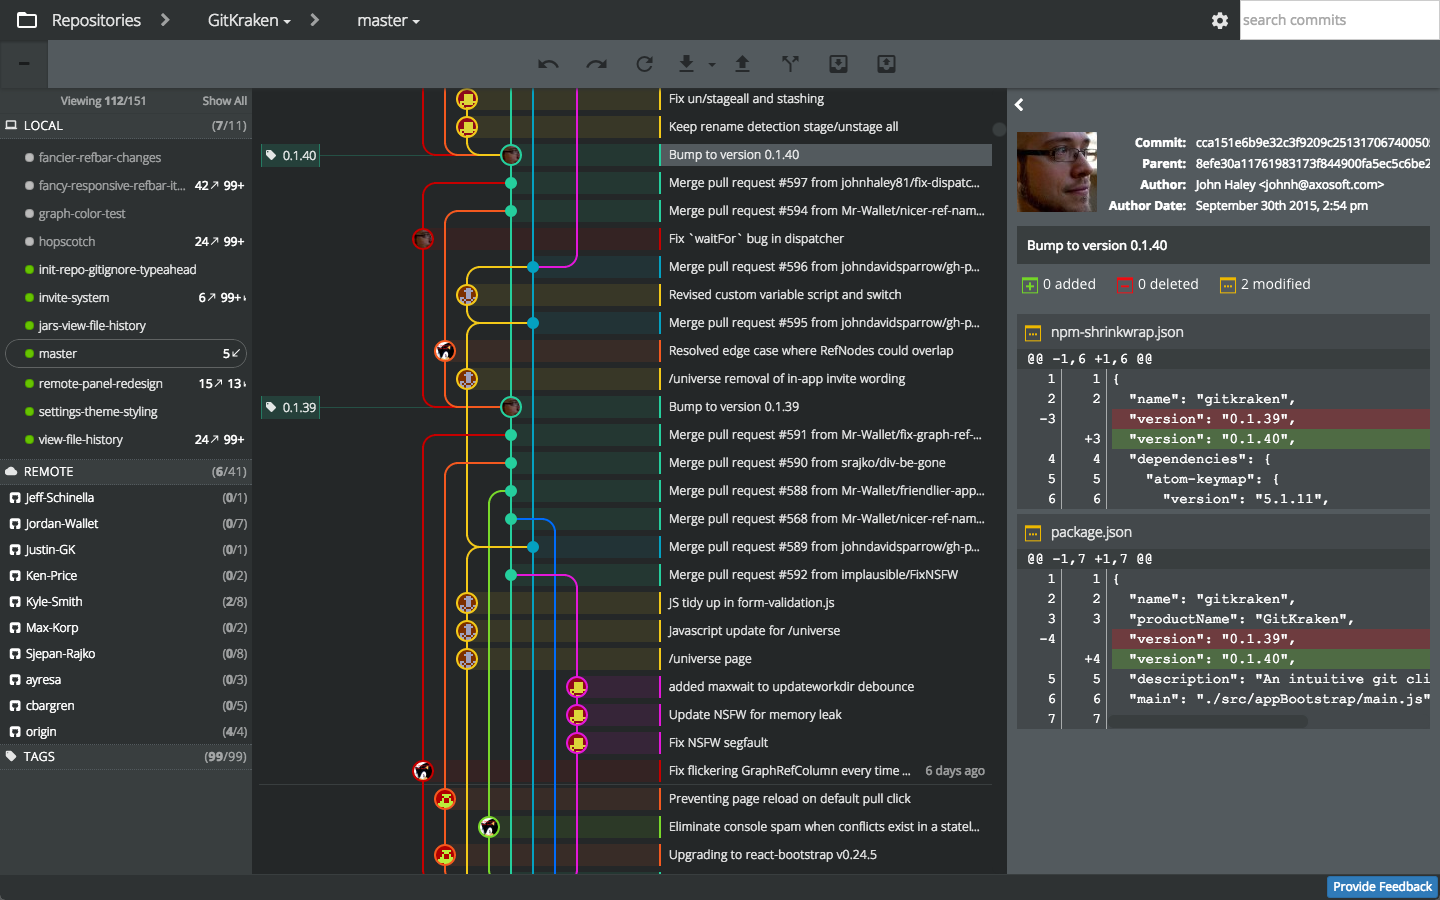
\includegraphics[width=0.8\linewidth]{Figures/introduction/gitkraken_main.png}
  \caption{Screenshot of the main view in GitKraken}
  \label{fig:gitkraken_main}
\end{figure}

In January of 2018, the Gnome project released a replacement for Gitk.
Gitg, shown in Figure~\ref{fig:gitg_screenshot}, is the git GUI client
for the Gnome environment.
The visualization is relatively clean, and it is able to produce a
visualization of the Linux repository quickly.
Like in Gitk, Gitg uses arrows to indicate that a branch has been cut.
Unlike in Gitk, the arrows do not hyperlink which makes it difficult to
find the parents of a commit.
There is no apparent way to find the other side of the branch,
as the interface does not provide information about the parents or
children of the commit.

\begin{figure}[htpb]
  \centering
  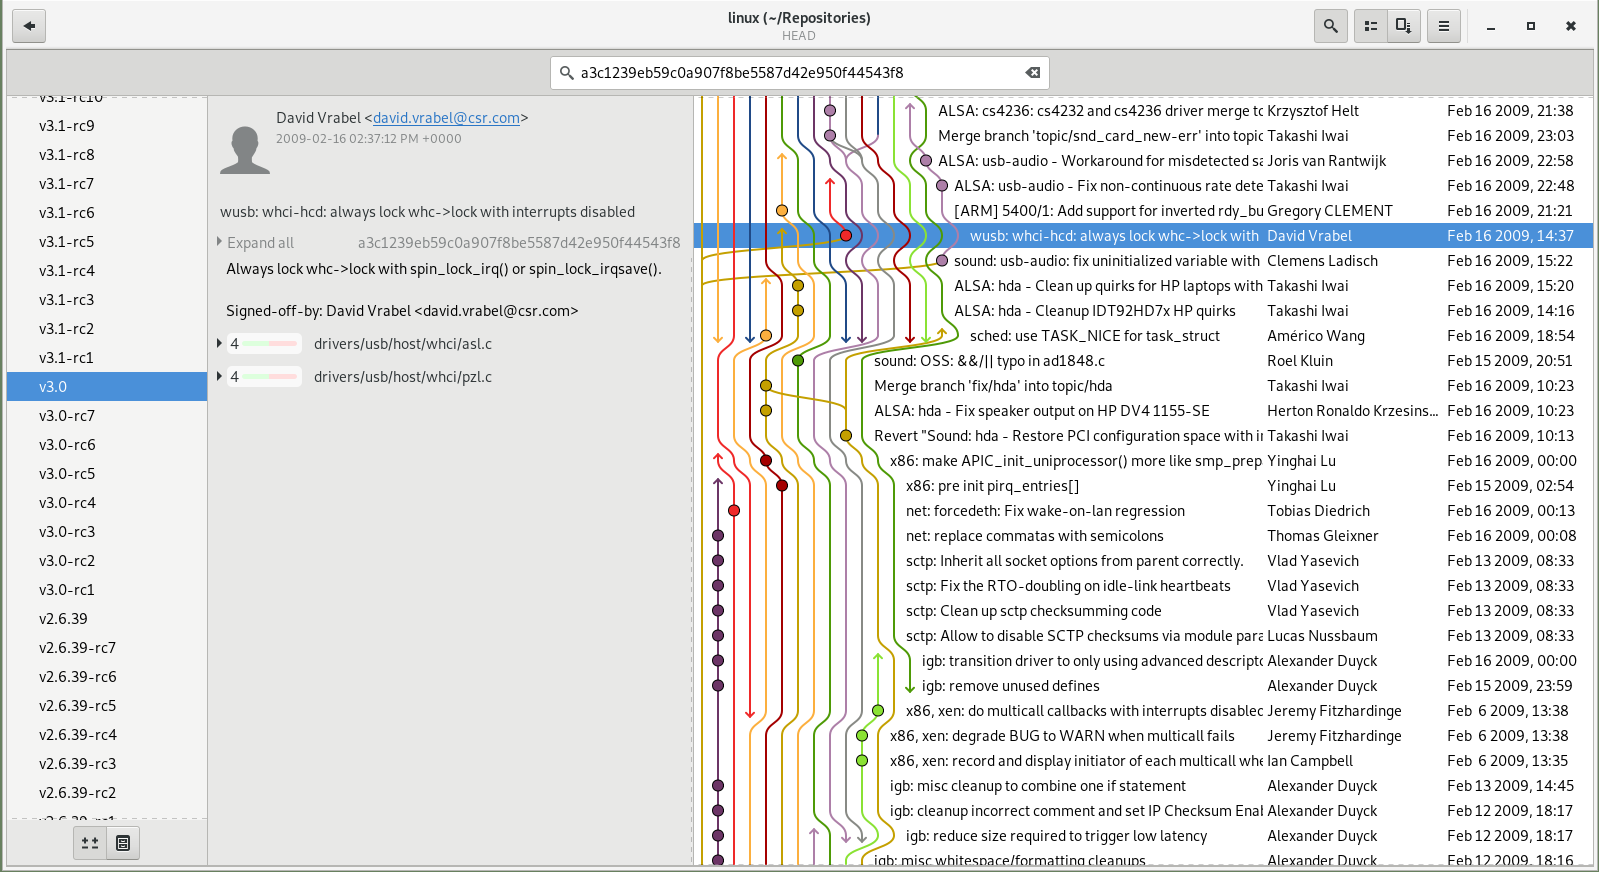
\includegraphics[width=0.8\linewidth]{Figures/introduction/gitg.png}
  \caption{Gitg interface from the Gnome project}
  \label{fig:gitg_screenshot}
\end{figure}

Giteye and most of the other visualizations are relatively
conventional, simply cleaning up the interface of Gitk.
GitLab and GitHub are both online repository hosts, with
visualization and summarization provided as well. While the GitLab
visualization does not appear to provide any additional information, the
visualization provided by GitHub takes advantage of additional internal
knowledge to display information about forks. Through this
visualization, GitHub displays the branch history of the repository
network, including the branches of the main repository and forks from
that.

With the exception of Gitk and Gitg, no GUI visualizers
are able to produce a visualization for the Linux repository, due to its
size: the GitHub visualizer displays an error message, stating that
there are too may forks to display; the GitKraken interface will freeze
and eventually crash while trying to load the repository; Giteye
and the other visualizers will consume all of the system memory before
they are able to produce a visualization. The Gitk interface is the
least polished, but is able to produce a visualization of the
repository.

\begin{figure}[htpb]
  \centering
  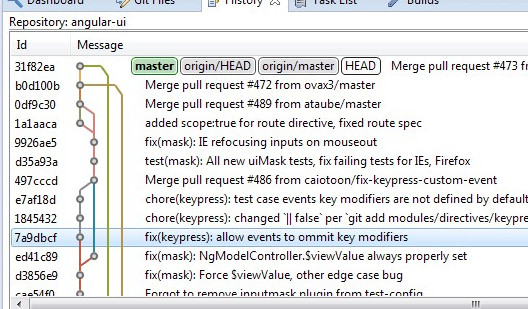
\includegraphics[width=0.8\linewidth]{Figures/introduction/giteye_graph.jpg}
  \caption{Screenshot of Giteye DAG view of a repository}
  \label{fig:giteye_screenshot}
\end{figure}

\begin{figure}[htpb]
  \centering
  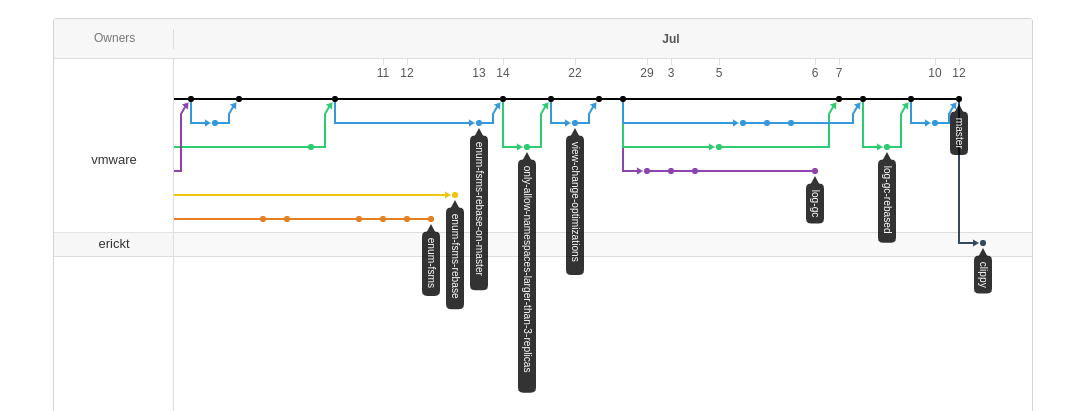
\includegraphics[width=0.8\linewidth]{Figures/introduction/github_dag.png}
  \caption{GitHub online network view of a repository}
  \label{fig:github_dag_screenshot}
\end{figure}

\begin{figure}[htpb]
  \centering
  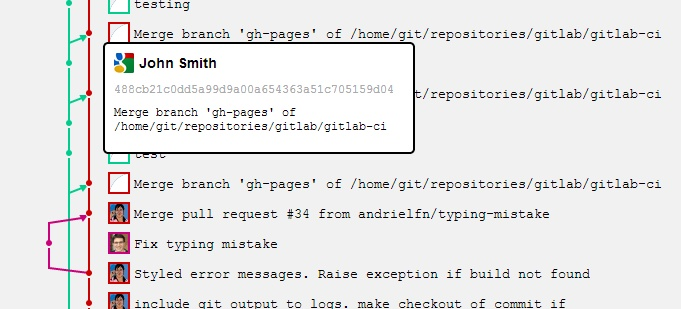
\includegraphics[width=0.8\linewidth]{Figures/introduction/gitlab_graph.jpg}
  \caption{GitLab online graph view}
  \label{fig:gitlab_dag_screenshot}
\end{figure}

\section{Git}
\label{sec:git}

% Commits;
Commits are the core of git repositories, storing the patch
representing the changes being made to the files in the repository, and
metadata about when the change was made, and who made the change.
In the metadata, commits store an author, an authordate, a committer,
and a commit date, and an ordered parent list of the commit hashes.
The author is the person who first created the patch and issued the
commit command.
The author date is when the commit was first created.
The committer and commit date contain the person who most recently
updated the commit, and when that update was made.
This metadata is exemplified in Figure~\ref{fig:commit_metadata} for a
commit and merge.

\begin{figure}[htpb]
  \centering
  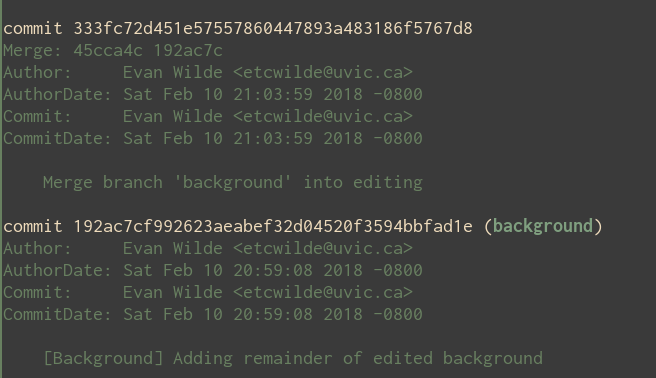
\includegraphics[width=0.8\linewidth]{Figures/background/commit_metadata.png}
  \caption{Screenshot of commit metadata for a commit and merge in the
    repository of this \paper{}.}
  \label{fig:commit_metadata}
\end{figure}

Commits are immutable; a commit cannot be modified once created.
When an update is made, new commit is created, the original metadata is
copied to the new commit, the relevant changes are made, the comitter
and commit date are updated, and the original commit is deleted.
If other commits the modified commit as one of their parents, they
are updated in the same manner to reflect the changes made .
This happens recursively until all descendants of the original commit
have been updated to reflect the new commit hash.

The patch contains the changes being made, including the
filenames, the line numbers, and the actual change, as shown in
Figure~\ref{fig:commit_patch}

Rebasing will also change the committer and commit date.

\begin{figure}[htpb]
  \centering
  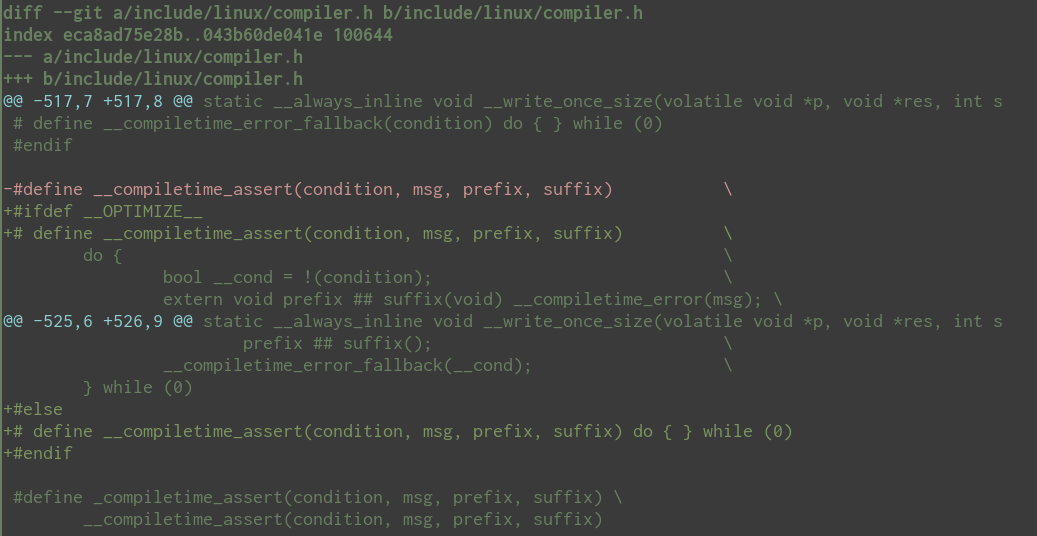
\includegraphics[width=0.8\linewidth]{Figures/background/commit_patch.png}
  \caption{Example of a commit patch from the Linux kernel repository
    from commit \textit{c03567a8e8d5}.}
  \label{fig:commit_patch}
\end{figure}

The parents of a commit are the next commits toward the initial commit.
The first parent in the list is the commit that is on the same branch
as the commit that is being created, i.e, the branch that the other
branches are being merged into.
The remaining commits are the branches being merged, in the order that
they are specified in the merge.
A non-merging commit will only have one parent.

To clarify the difference, non-merging commits are referred to as
commits and merging commits as merges.
In the scope of this thesis the term, repository event or simply event
is used to refer to either a commit or a merge.

% Integration;
Integration is the process by which the changes in a commit are
propagated to the master repository.
A small change with few dependencies is easier to integrate than changes.
Many times, Small changes that are localized contain bug fixes or small
changes to documentation.
An example of this from the Linux repository is shown in
Figure~\ref{fig:single_commit_merge}.

\begin{figure}[htpb]
  \centering
  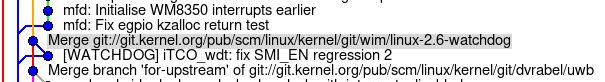
\includegraphics[width=0.8\linewidth]{Figures/background/single_commit.png}
  \caption{Example of a merge that only integrates a single commit}
  \label{fig:single_commit_merge}
\end{figure}

Major changes may be broken down into smaller segments and committed
seperately.
The set of these commits combined represent the full implmenentation of
the change,
which represents a logical separatation from the rest of the code, and
should be merged separately.
A set of major changes may be needed to implement an entire feature.
Each of these major changes may be merged into a feature branch before
being integrated into the project.

The Linux kernel repository has many examples of merge nesting like this.
In the Linux kernel, it is customary to have commits related to a single
subsystem in a single merge.
The subsystem may then be broken into sub-subsystems, for which there
are corresponding merges.
These merges contain the changes that modify the specific sub-subsystem.

For example, in the Linux repository, there is usually a merge
into the master branch of the repository for the changes to
the networking subsystem for a given release.
Within this merge, there are merges for wireless networking, Bluetooth,
and Ethernet, among other implementations of computer networking.
In this form, the merges act in a similar manner to directories in a
file system, where commits are the files containing the code, and merges
are the directories containing related files.
In this metaphor, the goal is to identify the file path to a given file,
and the other files that are in the same directory.
The root directory of the file path is the equivalent metaphorical
equivalent of the master branch.
To understand how a commit is integrated, it is necessary to understand
the merges that the commit was propagated through, and which commits are
integrated with it.
In order for a commit to be integrated, it must be propagated to the
master branch.
Merging commits is the process of integrating them.
The other commits that are merged with the commit are also necessary for
the given commit to be integrated in a meaningful way.

\section{Directed Acyclic Graph}
\label{sec:directed_acyclic_graph}

To allow for the flexibility needed for a distributed version control
system, git uses a \define{directed acyclic graph}{DAG} to model the
relationship between events.
The repository events make up the nodes in the graph, and the
child-parent\evan{no, the child has a list of references to it's
  parents, not the other way around.} relationship represents the edges.
Commits will have a single parent, which is the repository event that
is at the head of the current branch at the time that the commit
is created.
Merge nodes have an ordered list of
parents\footnote{It is possible for a merge to have many parents, commit
  2cde51fbd0f3 has 66 parents},
each parent is the head of each branch being merged.
The first parent is the head of the current branch, and the other
parents are the heads for the other branches being merged, in the order
that they are specified in the merge command.
Every repository will have at least one initial commit, which
will have no parents, but it is possible for repositories to have
multiple initial commits.
Furthermore, it is possible for the graph of a repository to be
disconnected; disconnected branches are refered to as orphaned branches
with respect to the rest of the graph \evan{They are with respect to
  each other and all other branches in the repository. The documentation
  doesn't say much on this topic}.


The model is simple, but flexible.
The flexibility of the model makes it more difficult to reason about,
stricter models are easier to reason about since the model must follow
more rules.

For example, many version control systems have a well-defined notion of
the master branch.
In SVN, this is referred to as the ``trunk'' branch.
There is a single trunk branch, and it is well-defined, it won't be
confounded with another branch.
The DAG model in git does not explicitly define a master branch, or even
enforce the requirement that one exists.
Instead, the idea of the master branch is a social construct used to
identify where releasable code should be merged into, and where the
final product will be released from.
This relies on the discipline of the people committing code to the
repository to maintain a well-defined master branch.

The convention in git is that the first parent of the current commit was
made to the same branch as the commit. Using this definition it is
possible to define the set of commits in the branch as those that are
long the first-parent path up to the first place where the first-child
of the first-parent is not a commit of the branch.
Using the example in Figure~\ref{fig:repoEvents2}, branch B consists of
nodes 6, 4, and 2. Branch A consists of nodes 7, 5, 3, and 1.


\begin{figure}[htbp]
  \centering
  \resizebox{0.5\textwidth}{!}{
  \begin{tikzpicture}[auto, on grid, semithick, state/.style={circle, text=black}]
    \foreach \x in {0, 1, 2, 3}
    \draw[shift={(\x + 0.5, -0.5)}, color=black] (0cm, 2cm) -- (0pt, -0.2cm);

    \node[state, draw=chartblue] (1) {1};
    \node[state, draw=chartyellow, above right=of 1] (2) {2};
    \node[state, draw=chartblue, right=of 1] (3) {3};
    \node[state, draw=chartyellow, right=of 2] (4) {4};
    \node[state, draw=chartblue, right=2cm of 3] (5) {5};
    \node[state, draw=chartyellow, right=of 4] (6) {6};
    \node[state, draw=chartblue, right=of 5] (7) {7};

    \draw (2) edge[-stealth, chartyellow] (1);
    \draw (4) edge[-stealth, chartyellow] (3) edge[-stealth, chartyellow] (2);
    \draw (6) edge[-stealth, chartyellow] (4);

    \draw (3) edge[-stealth, chartblue] (1);
    \draw (5) edge[-stealth, chartblue] (3) edge[-stealth, chartblue] (4);
    \draw (7) edge[-stealth, chartblue] (5) edge[-stealth, chartblue] (6);

    \node[rectangle, black, text=black, above=of 6] (branchB) {B};
    \draw (branchB) edge[black] (6);

    \node[rectangle, black, text=black, above=2cm of 7] (branchA) {A};
    \draw (branchA) edge[black] (7);

    \foreach \x in {0, 1, 2, 3, 4}
      \node[shift={(\x, -0.6)}, color=black] {$t_\x$};
  \end{tikzpicture}
}
  \caption{A small example of a sequence of commits and merges.
    The branch pointer A reference commit 7, which merges the head of
    branch B, commit 6, into the original head of branch A, which was
    commit 5. Merge 7 is the most recent change to the repository.}
  \label{fig:repoEvents2}
%\vspace{-3mm}
\end{figure}


Git has no internal safe-guards to protect branches from obfuscation.
When certain conditions are met, it is possible to perform an action on
the repository which results in commits to appear as if they were
performed as part of a different branch.
The series of steps to swap branches is called a foxtrot\footnote{See
  \url{http://bit-booster.blogspot.ca/2016/02/no-foxtrots-allowed.html}
  for a full description of the issue}.

It is necessary for multiple repositories to be interacting for a
foxtrot to occur.
The following is a short example of the series of steps in the foxtrot,
also shown in Figure~\ref{fig:FoxtrotSteps}.
Bob and Alice have both made local clones of a remote
repository and are making changes to the master branch of their local
repository.
Bob and Alice both make local changes to the same file in the
repository and commit those changes into the same branch.
Alice pushes her changes to the repository first, which results in a
fast-forward merge of the remote branch.
Alice's commit is clearly pushed to the master branch.
Bob attempts to push, but the push fails as his repository is not in
sync with the remote branch anymore, so Bob pulls.
The pull merges the difference in the remote branch into the local
branch.
Alice and Bob edited the same file creating a merge conflict, so Git
cannot perform a fast-forward merge.
Bob resolves the conflict and a merge commit is created to store the
resolution.
The head of Bob's local branch at the time of the pull is the first
parent of this merge commit, and the changes made by Alice are the
second parent.
With the merge conflict resolved, Bob pushes the changes back to the
remote branch.
Prior to Bob pushing his changes to the remote repository, Alice's
commit was at the head of the master branch.
After Bob's push, this information is lost, and it appears that Alice's
commit was merged into the master branch by Bob.
This sequence of operations swaps the branches: the commits that were in
remote's master now appear to be made to a separate branch and merged
into the master branch, while Bob's commits appears as if they were made
to the master branch.
The merge commit that merges the remote master branch into Bob's master
branch is the foxtrot merge.


\begin{figure}[htbp]
  \begin{tabulary}{\textwidth}{LLL}
    Alice's Repo. & Origin Repo. & Bob's Repo.\\
    \tiny{
    Alice has made a local clone of the remote repository
    \textit{Origin}.}
    &
    &
    \tiny{Bob has made a local clone of the remote repository
    \textit{Origin}.}
    \\
    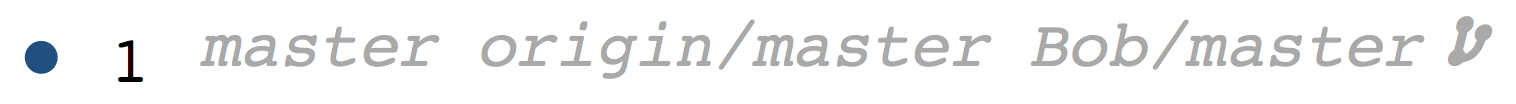
\includegraphics[width=0.27\textwidth]{Figures/background/foxtrot/alice_1.png} &
    
\includegraphics[width=0.27\textwidth]{Figures/background/foxtrot/origin_1.png} &
    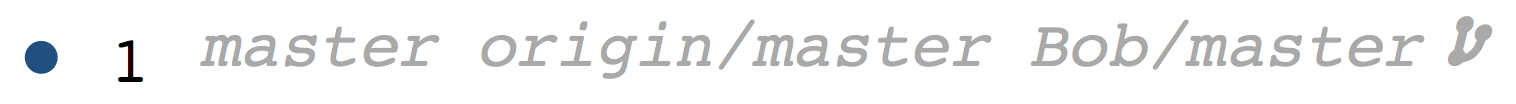
\includegraphics[width=0.27\textwidth]{Figures/background/foxtrot/alice_1.png} \\

    \tiny{Alice makes some changes and commits them to her local repository.}

    &
    &
    \tiny{Bob makes some changes to the same file as Alice and commits them in
    his local repository.}
    \\

    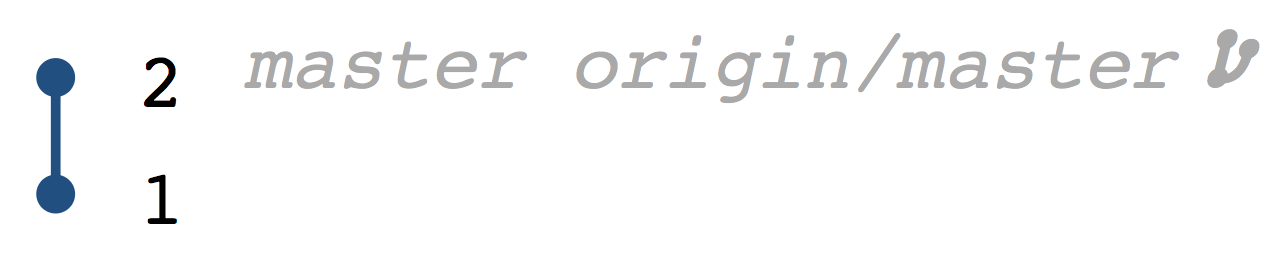
\includegraphics[width=0.27\textwidth]{Figures/background/foxtrot/alice_2.png} &
    
\includegraphics[width=0.27\textwidth]{Figures/background/foxtrot/origin_1.png} &
    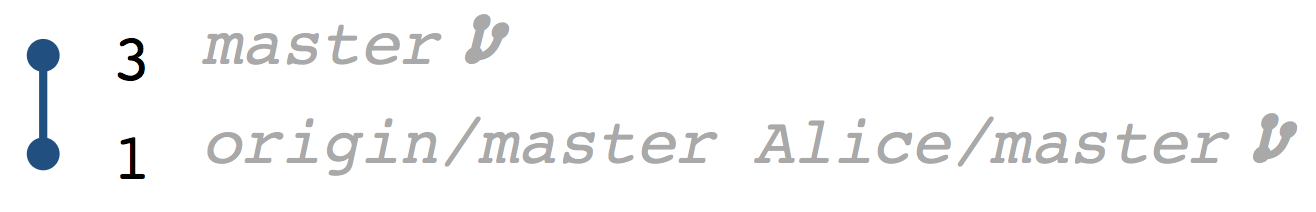
\includegraphics[width=0.27\textwidth]{Figures/background/foxtrot/bob_2.png} \\

    \tiny{Alice pushes her changes back into the master branch of the remote
    repository.} &
    \tiny{The remote repository reflects the push by fast-forward merging
    Alice's master branch into the remote master branch.} &
    \tiny{Bob is not made aware of these changes yet.} \\


    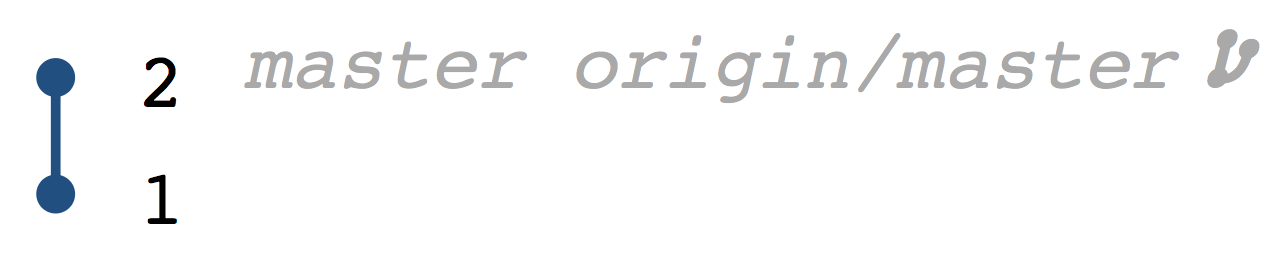
\includegraphics[width=0.27\textwidth]{Figures/background/foxtrot/alice_2.png} &
    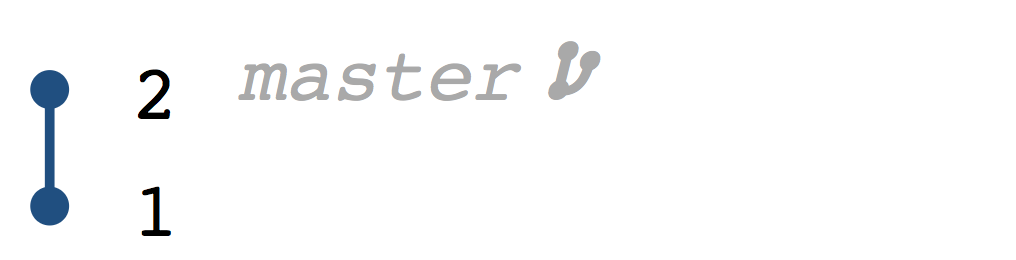
\includegraphics[width=0.27\textwidth]{Figures/background/foxtrot/origin_2.png} &
    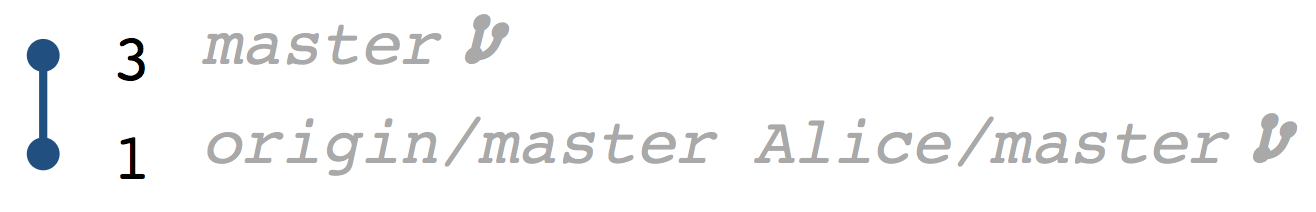
\includegraphics[width=0.27\textwidth]{Figures/background/foxtrot/bob_2.png} \\

    &
    &
    \tiny{Bob attempts to push, but this results in a merge conflict.}
    \\

    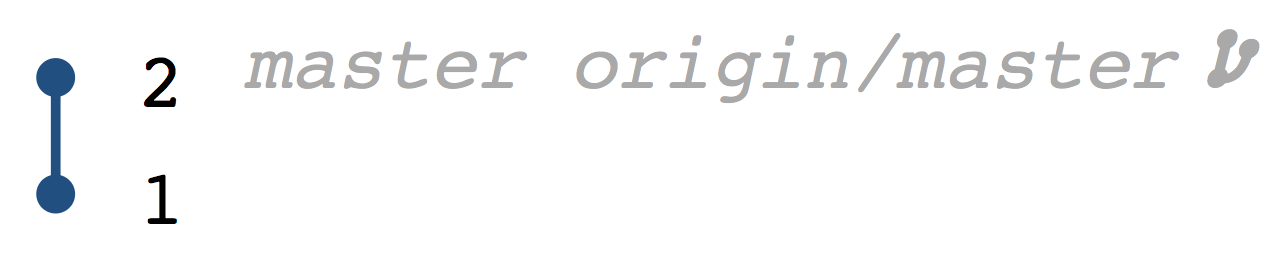
\includegraphics[width=0.27\textwidth]{Figures/background/foxtrot/alice_2.png} &
    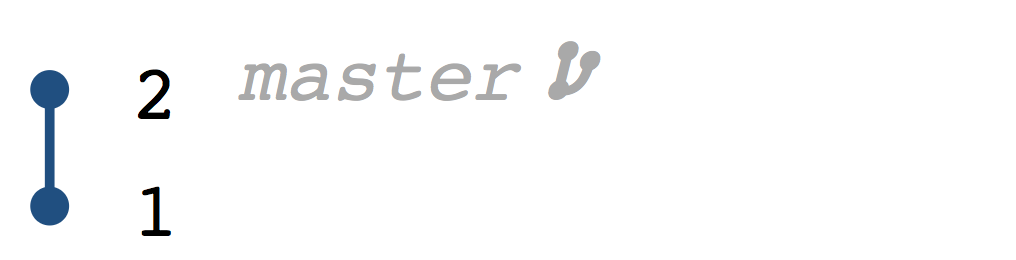
\includegraphics[width=0.27\textwidth]{Figures/background/foxtrot/origin_2.png} &
    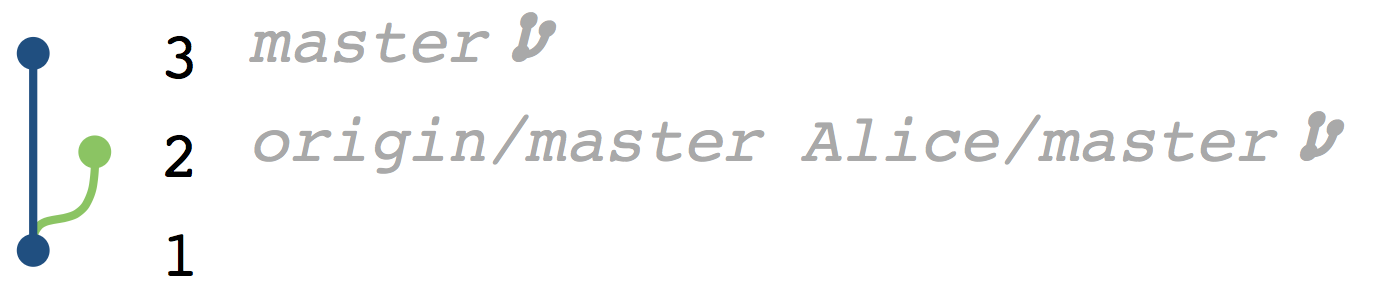
\includegraphics[width=0.27\textwidth]{Figures/background/foxtrot/bob_3.png} \\

    &
    &
    \tiny{Upon fixing the merge conflict, the pull merges the remote master
    branch into Bob's master branch.}
    \\

    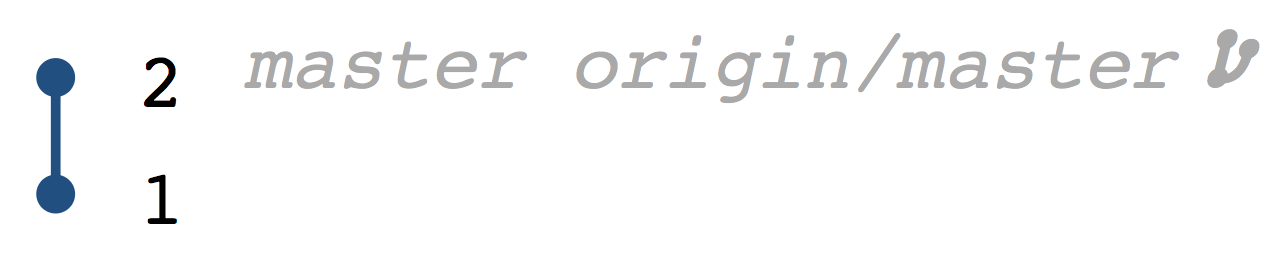
\includegraphics[width=0.27\textwidth]{Figures/background/foxtrot/alice_2.png} &
    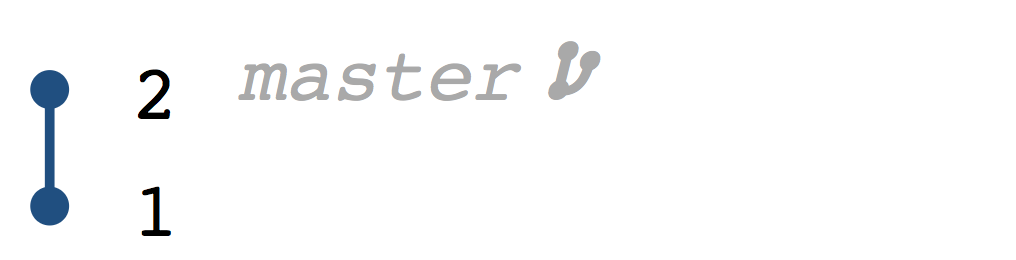
\includegraphics[width=0.27\textwidth]{Figures/background/foxtrot/origin_2.png} &
    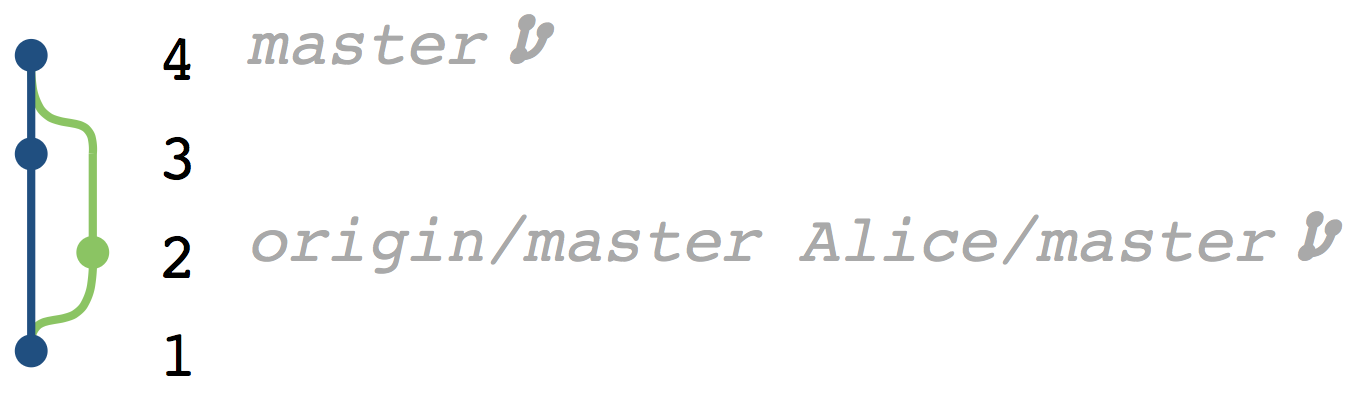
\includegraphics[width=0.27\textwidth]{Figures/background/foxtrot/bob_4.png} \\

    &
    \tiny{Bob's changes are pushed to the remote.}
    &
    \\

    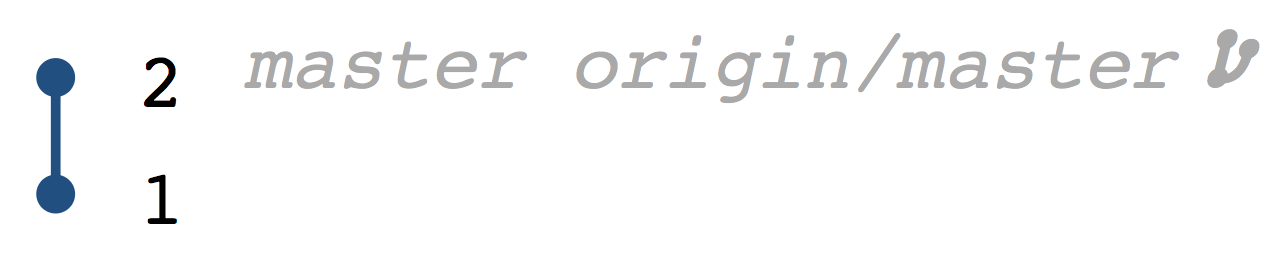
\includegraphics[width=0.27\textwidth]{Figures/background/foxtrot/alice_2.png} &
    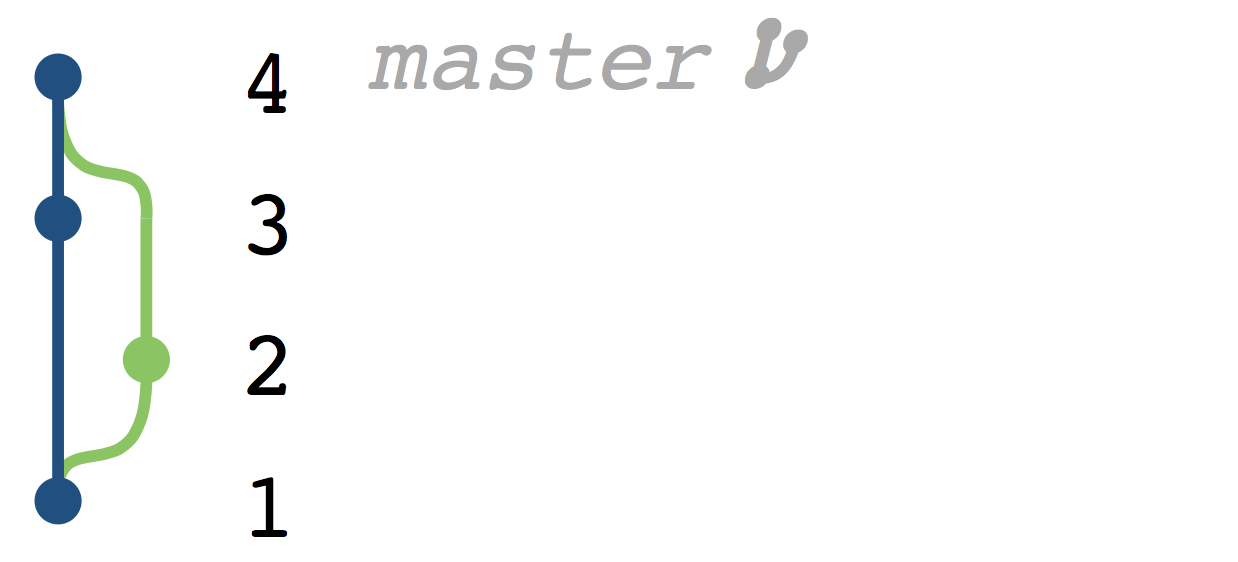
\includegraphics[width=0.27\textwidth]{Figures/background/foxtrot/origin_3.png} &
    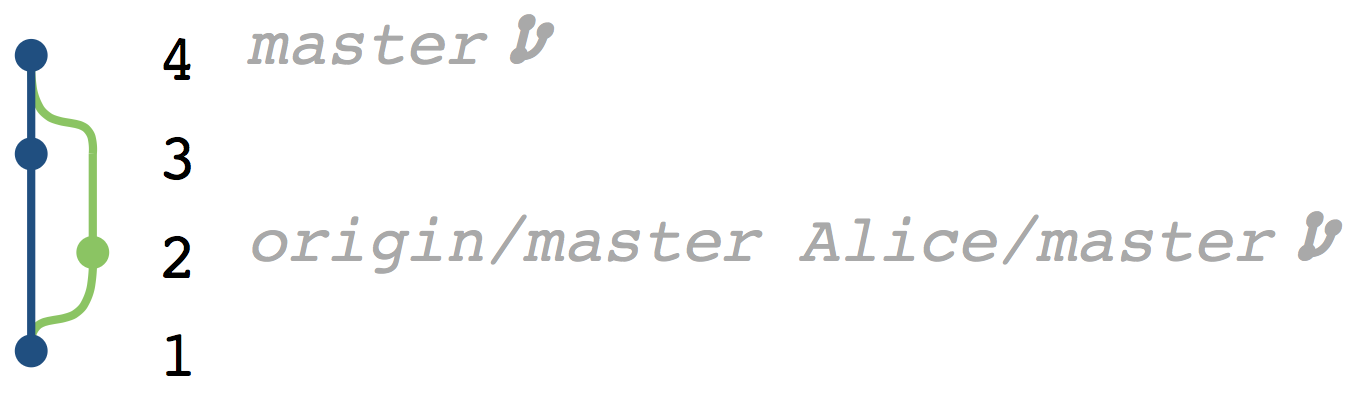
\includegraphics[width=0.27\textwidth]{Figures/background/foxtrot/bob_4.png} \\

  \end{tabulary}
  \caption{The sequence of steps that are part of the foxtrot, from the
  point of view of each repository. Alice's commit is pushed to the
  master branch, but as a result of the foxtrot, in the end appears to
  be merged into the master branch.}
  \label{fig:FoxtrotSteps}
\end{figure}

The effect of this can have different repercussions depending on the
project.
In the best case, the repository visualizations will not give an
accurate visualization of how commits were integrated into the project,
which may lead to confusion.
In a more serious situation, a specific branch is considered to be the
stable branch, where only code that has been reviewed and tested is
accepted.
When a regression occurs, the project may need to revert back to a
previous stable state, where the regression is not present.
This requires the ability to find and track the master branch, which may
be confounded by a foxtrot.
Picking the incorrect commit to revert to could lead to serious
consequences.
In the Linux project, the merges to the master branch are
the code that Linus has reviewed and accepted into the mainline kernel.
\evan{I don't think he writes much code anymore, it looks like he mostly
  merges things that have been reviewed.}

As mentioned earlier, the nodes in the DAG are immutable;
once a commit or merge is created, it cannot be changed.
Git allows operations to alter the events and re-order them,
but this will create a new event with a new commit hash.
This property makes it impossible for nodes to store information about
their children, and in extension, how the commit is being merged, as
this information is not available when the commit is created.
Git provides the command \verb|git log --children|, which traverses the
DAG and inverts the edges.
The next child that is a merge is the first merge on the path to being
integrated.

The graph combined with the child information gives most of the
information necessary for understanding how the commit is
merged into the master branch; however, information about the specific
merge into the master branch is still missing.
Furthermore, the graph itself is not always easy to understand, as shown
in Figure~\ref{fig:git_graphs}.
This figure contrasts the levels of complexity that can be found in a
given section of the Linux kernel repository.

\begin{figure}[htpb]
  \centering
  \begin{subfigure}[b]{0.8\textwidth}
    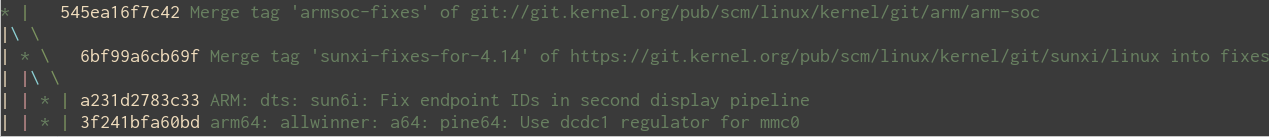
\includegraphics[width=\textwidth]{Figures/background/git_graph.png}
    \caption{In the simple case, it is relatively easy to see
      that \textit{a231d} is merged into \textit{6bf99},
      which is then merged into \textit{545ea}.}
    \label{fig:trivial_graph}
  \end{subfigure}

  \begin{subfigure}[b]{0.8\textwidth}
    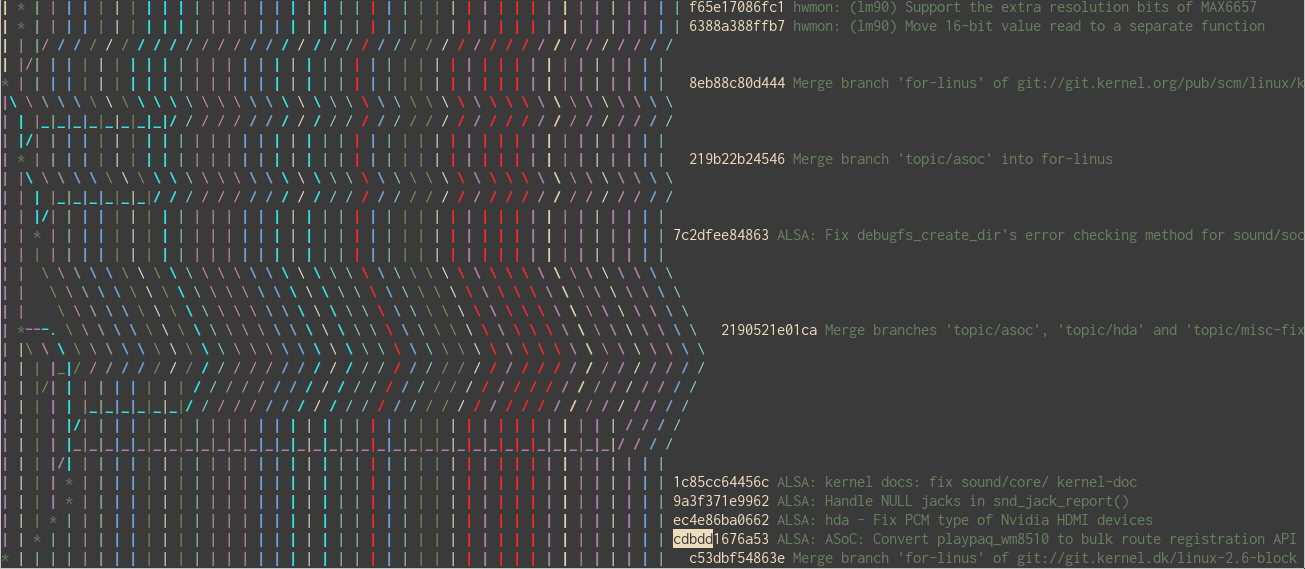
\includegraphics[width=\textwidth]{Figures/background/git_graph_complex.png}
    \caption{As the number of merges that a commit passes through
      increases, it becomes more challenging to understand how the
      commit is integrated.}
  \end{subfigure}
  \caption{The git graph visualization of two sections of the Linux
    repository.}
  \label{fig:git_graphs}
\end{figure}

Most repositories are simple enough that it is possible to identify how
commits are integrated using the visualizations of the DAG that are
available with the current tools.
Difficulties arise in larger repositories.
The master branch can be confounded due to \foxtrot{}
merges, making it difficult to identify merges to the master branch.
Sheer number of commits being added to various branches at a given
time can make it difficult to understand which branch a commit is
being added to.

\section{Linux}\label{sec:linux}

This \paper{} studies and proposes a visualization for the Linux kernel
repository.
The repository itself is complex, contain tens of thousands of commits
and thousands of merges per year.
Older versions of the kernel are used in a wide
variety of situations including various Linux desktop distributions,
IOT device firmware, web servers,
spacecrafts\footnote{Linux is used heavily at SpaceX
  \url{https://lwn.net/Articles/540368/}}, and in mobile devices as the
kernel of the Android platform.
These kernels are sometimes modified forks of the official Linux kernel,
made to be more suitable for the specific needs of the application.
Due to these application-specific modifications,
it is not feasible to update to the latest version of the
kernel.
While it may not be feasible to update, the changes being made to the
official version are necessary as they fix bugs, patch security
issues, and improve performance.
Due to the sometimes critical nature of
the patches being merged into the current version of the kernel, it is
necessary for maintainers working on an application-specific fork of the
kernel to sift through the commits coming into the official version,
looking for changes that may impact the kernel that they are
maintaining.


% This section presents statistics on the dataset collected from the Linux
% repository. Included is information about the number of authors,
% commits, and merges per release, as well as the range of dates from
% which the data was collected. This information is useful for
% characterizing the problem, and understanding how to best group the
% commits in a way that is useful and easy to understand.
